%
% THIS TEMPLATE DEVELOPED BY STEPHEN MCKIM (2009), UPDATED BY ROBERT GRANDIN (2011)
%
% COMMENTS REGARDING THE FUNCTIONALITY PROVIDED BY VARIOUS COMMANDS AND OPTIONS
% CAN BE FOUND THROUGHOUT THE DOCUMENT.  FOLLOWING THE DOCUMENT ITSELF ARE
% REFERENCE COMMANDS WHICH MAY BE USEFUL.  THESE REFERENCE COMMANDS ARE WITHIN
% A MASSIVE COMMENT BLOCK TO AVOID AFFECTING THE DOCUMENT.  AS SUCH, THEY MAY
% BE LEFT IN-PLACE DURING DOCUMENT GENERATION/PREPARATION.
%
\documentclass[12pt, letterpaper]{article}
% 'article' CAN BE REPLACED WITH 'report' or 'book'
%     -- ARTICLE DOES NOT RECOGNIZE \chapter OR \part
%        -- \section IS THE HIGHEST LEVEL ALLOWED
%        -- WELL-SUITED FOR SHORT DOCUMENTS (E.G., HOMEWORK ASSIGNMENTS)
%     -- report AND book ALLOW \chapter AND \part
%     -- book ADDS BLANK PAGES BETWEEN PARTS AND PAGE HEADER INFORMATION


% =============================================================================
% ========
% ========			PREAMBLE / DOCUMENT SETUP
% ========
% =============================================================================


% PACKAGES TO BE USED
\usepackage{array}				% ARRAYS
\usepackage[latin1]{inputenc}	% LATIN INPUT-ENCODING TO ALLOW USE OF ACCENTED
%								% CHARACTERS IN LATIN-DERIVED LANGUAGES (E.G.,
%								% ENGLISH, SPANISH).  THIS CAN BE OPERATING SYSTEM-
%								% DEPENDENT:
%								% 		LINUX: 		latin1
%								%		WIN:		ansinew
%								% 		MAC: 		applemac
\usepackage{pdflscape}			% ALLOW LANDSCAPE ENVIRONMENTS. pdflscape WILL 
%								% ROTATE IMAGES TO APPEAR NORMALLY WHEN VIEWING 
%								% THE PDF FILE (I.E. YOU DON'T HAVE TO ROTATE 
%								% YOUR HEAD TO VIEW THE FIGURE/TABLE)
\usepackage{fontenc}			% OUTPUT-ENCODING FOR CORRECT RENDERING OF 
%								% CHARACTERS.  NO [] OPTION NEEDED FOR LATIN-
%								% BASED LANGUAGES AND GREEK CHARACTERS.  OUTPUT
%								% OF NON-LATIN LANGUAGES COULD BE INCORRECT.
\usepackage{amsmath,amssymb,amsthm}	% MATH TOOLS/SYMBOLS AND GREEK ALPHABET
\usepackage{graphicx}			% GRAPHICS/FIGURE MANIPULATION
\usepackage{subfigure}			% MULTIPLE GRAPHICS IN A SINGLE FIGURE
\usepackage{fullpage}			% USE THE FULL PAGE FOR CONTENT.  DEFAULTS TO 
%								% 1-INCH MARGINS ON ALL SIDES.
\usepackage{longtable}			% ALLOW FOR TABLES TO SPAN MULTIPLE PAGES.
\usepackage{nomencl}			% AUTOMATIC GENERATION OF NOMENCLATURE
\usepackage{float}				% ALLOW DECLARATION OF CUSTOM 'FLOAT' OBJECTS (IN
%								% ADDITION TO THE STANDARD FIGURES AND TABLES).
%								% 'FLOATS' CANNOT BE SPLIT-UP OVER PAGE BREAKS.
\usepackage{hyperref}			% HYPERLINKED URLS
\usepackage{breakurl}     		% ALLOW URL'S TO BREAK AS NECESSARY TO WRAP TO 
								% THE NEXT LINE.
\usepackage{makeidx}			% GENERATION OF AN INDEX
\usepackage{natbib}				% GENERATION OF A BIBLIOGRAPHY
%\usepackage{apacite}			% APA-FORMATTED CITATIONS
\usepackage{moreverb}			% ALLOW FOR LINE NUMBERS BESIDE TEXT IN VERBATIM 
%								% ENVIRONMENT
\usepackage{color}				% ALLOW COLOR 
\usepackage{listings}			% AUTOMATIC SYNTAX HIGHLIGHTING IN ENVIORONMENTS
%								% DEMARKATED BY \begin{lstlisting} AND
%								% \end{lstlisting}
\lstset{ %						% OPTIONS FOR SYNTAX HIGHLIGHTING
	language=C++,	            % CHOOSE THE LANGUAGE OF THE CODE
	basicstyle=\footnotesize,   % THE SIZE OF THE FONTS USED FOR THE CODE
	numbers=left,               % WHERE TO PLACE THE LINE-NUMBERS
	numberstyle=\footnotesize,  % SIZE OF THE FONTS USED FOR THE LINE-NUMBERS
	stepnumber=1,               % THE STEP BETWEEN TWO LINE-NUMBERS.  IF IT IS
%								% 1, EACH LINE WILL BE NUMBERED, 2 WILL BE
%								% EVERY-OTHER LINE, ETC.
	numbersep=5pt,              % DISTANCE BETWEEN LINE-NUMBERS AND CODE
	backgroundcolor=\color{white},  % SET THE BACKGROUND COLOR.  REQUIRES
%								% \usepackage{color} ABOVE
	showspaces=false,           % SHOW SPACES BY ADDING UNDERSCORES
	showstringspaces=false,     % UNDERLINE SPACES WITHIN STRINGS
	showtabs=false,             % SHOW TABS WITHIN STRINGS USING UNDERSCORES
	frame=single,	            % ADDS A FRAME AROUND THE CODE
	tabsize=4,	                % SETS DEFAULT TABSIZE (NUMBER OF SPACES)
	captionpos=b,               % SETS CAPTION POSITION TO BOTTOM
	breaklines=true,            % SETS AUTOMATIC LINE BREAKING
	breakatwhitespace=false,    % SETS IF AUTOMATIC BREAKS SHOULD ONLY HAPPEN
%								% AT WHITESPACE
	title=\lstname,            	% SHOW THE FILENAME OF FILES INCLUDE WITH
%								% \lstinputlisting;
%								% ALSO TRY CAPTION INSTEAD OF TITLE
	escapeinside={(*@}{@*)},    % FOR COMMENTS WITHIN CODE THAT YOU DO NOT WANT
%								% TO APPEAR IN THE LISTING (E.G., LABELING LINES
%								% WITHIN A LISTING ENVIRONMENT FOR REFERENCING
%								% IN THE TEXT).
%	morekeywords={*,...}        % ADDITIONAL KEYWORDS TO BE ADDED TO THE
%								% DEFAULT LIST AS DEFINED BY language
}

% COMMENT-OUT THESE LINES IF NO INDEX IS NEEDED
%\documentstyle{makeidx}
\makeindex

% PDF FILE PARAMETERS.
\hypersetup{	
	% THESE FIRST THREE OPTIONS SHOULD BE UPDATED FOR EACH DOCUMENT/PROJECT.
	pdftitle={PDF TITLE},		% DOCUMENT TITLE
	pdfauthor={PDF AUTHOR},     	% DOCUMENT AUTHOR
	pdfsubject={PDF SUBJECT},  	% DOCUMENT SUBJECT
	%
	% THE FOLLOWING OPTIONS DO NOT REQUIRE MODIFICATION
	pdftoolbar=true,        	% SHOW ACROBAT'S TOOLBAR
	pdfmenubar=true,       		% SHOW ACROBAT'S MENU
	pdffitwindow=false,     	% WINDOW FIT-TO-PAGE WHEN OPENED
	pdfstartview={FitH},    	% FITS WIDTH OF PAGE TO THE ACROBAT WINDOW
	pdfnewwindow=true,      	% LINKS IN NEW WINDOW
	colorlinks=true,       		% FALSE: BOXED LINKS,    TRUE: COLORED LINKS
	linkcolor=red,          	% COLOR OF INTERNAL LINKS
	citecolor=green,        	% COLOR OF BIBLIOGRAPHICAL LINKS
	filecolor=magenta,      	% COLOR OF FILE LINKS
	urlcolor=blue           	% COLOR OF EXTERNAL LINKS
}

% NOMENCLATURE-GENERATION
% NOTE THAT 'OLD VERSION' AND 'NEW VERSION' REFER TO THE VERSION OF YOUR
% INSTALLATION OF THE nomencl PACKAGE.
%\makeglossary 	% OLD VERSION
\makenomenclature % NEW VERSION

% ADD DATE
%\date{2009-03-01}

% DEFINE ADDITIONAL COMMANDS AND OPTIONS
\renewcommand{\arraystretch}{1.3}
\newcommand{\U}[1]{\ensuremath{\, \mathrm{#1}}}
\newcommand{\ii}[1]{{\it #1}}
\newcommand{\nn}[1]{#1n}
\parskip=0.10in
\parindent=0pt

% THESE TWO LINES SETUP THE DEFINITION FOR THE \begin{definition} AND 
% \end{definition} TAGS (REQUIRED TO AVOID COMPILATION ERRORS).
\newenvironment{definition}[1][Definition]{\begin{trivlist}
\item[\hskip \labelsep {\bfseries #1}]}{\end{trivlist}}

% =============================================================================
% ========
% ========			THE ACTUAL DOCUMENT
% ========
% =============================================================================
\begin{document}

% =============================================================================
% ========
% ========			INTRODUCTORY / SUMMARY INFORMATION
% ========
% =============================================================================
% COMMENT-OUT LINES BELOW AS NECESSARY TO NOT INCLUDE FILES
\begin{titlepage}

\vspace*{5.5 cm}			% VERTICAL SPACE BETWEEN TOP OF PAGE AND THE NEXT
%								% ELEMENT (IN THIS CASE, THE TEXT OF THE TITLE)

\begin{center}				% CENTER THE TITLEPAGE ELEMENTS

	% THIS FILL-IN-THE-BLANK TITLEPAGE IS SETUP FOR HOMEWORK ASSIGNMENTS.  
	% MODIFY THIS DOCUMENT AS-NEEDED TO INCORPORATE THE FEATURES YOU NEED.
	\begin{LARGE}
		\textbf{\underbar{My Title}} \\
	\end{LARGE}
	\vskip 0.15 cm

	\begin{large}
		Course Number: Name
	\end{large}
	\vskip 0.2cm

	\begin{normalsize}
		My Name
		\vskip 0.6 cm
		\textbf{Date Submitted}
	\end{normalsize}
	

%	% TITLEPAGE ELEMENTS
%	\begin{LARGE}
%		\textbf{\underbar{Preliminary Design Review Report DRAFT}} \\
%	\end{LARGE}
%
%	\vskip 0.15 cm
%
%	\begin{large}
%		AerE 462: Senior Design
%	\end{large}
%	\vskip 0.2cm
%
%	\begin{LARGE}
%		\emph{Team Silent Sasquatch} \\[0.5 cm]
%	\end{LARGE}
%
%	\begin{normalsize}
%
%	Author 1 \\
%	Author 2 \\
%	Author 3 \\
%
%
%	\vskip 0.6 cm
%
%	\textbf{September 25, 2009}
%
%	\end{normalsize}

\end{center}


\end{titlepage}

\begin{titlepage}

% THIS 'EXECUTIVE SUMMARY' FUNCTIONS AS A SUMMARY OF THE REST OF THE DOCUMENT.
% IT CAN ALSO BE CALLED AN 'ABSTRACT'.

\begin{center}
	\begin{large}
		\textbf{Executive Summary}
		\vskip 0.2cm
	\end{large}
\end{center}

\begin{normalsize}

This is a wonderful executive summary blah blah blah.  Look, I am lots of pretty text that is formatted in goregeous LaTex font!

\end{normalsize}

\end{titlepage}

\printnomenclature	% PRINT NOMENCLATURE (NEW VERSION COMMAND)
% \printglossary 	% PRINT NOMENCLATURE (OLD VERSION COMMAND)
\tableofcontents
\listoffigures
\listoftables

% =============================================================================
% ========
% ========			THE "MEAT" OF THE DOCUMENT
% ========
% =============================================================================
% FORCE A NEW PAGE TO ENSURE THAT THE "MEAT" OF THE DOCUMENT BEGINS ON A NEW 
% PAGE AND NOT ON A PARTIAL PAGE SHARED BY THE SUMMARY INFORMATION
\newpage


\section{Index and Nomenclature}
This is a sample section and should be indexed as 'sample'
\cite{sample01}.  \index{sample}

There are also three nomenclature terms defined: $alpha$, $\gamma_{st}$, and
$\ddot{S}_1$.

\nomenclature{$\alpha$}{Angular Acceleration}
\nomenclature{$\gamma_{st}$}{Specific weight of steel}
\nomenclature{$\ddot{S}_1$}{Acceleration of bullet, Phase I}


\newpage 
\section{Figures}

Here is a sample image:
\begin{figure}[!ht]	% FORCE LOCATION TO HERE (h), OR TOP OF PAGE (t)
	\centering								% CENTER THE FIGURE

	% LINK TO THE ACTUAL IMAGE

	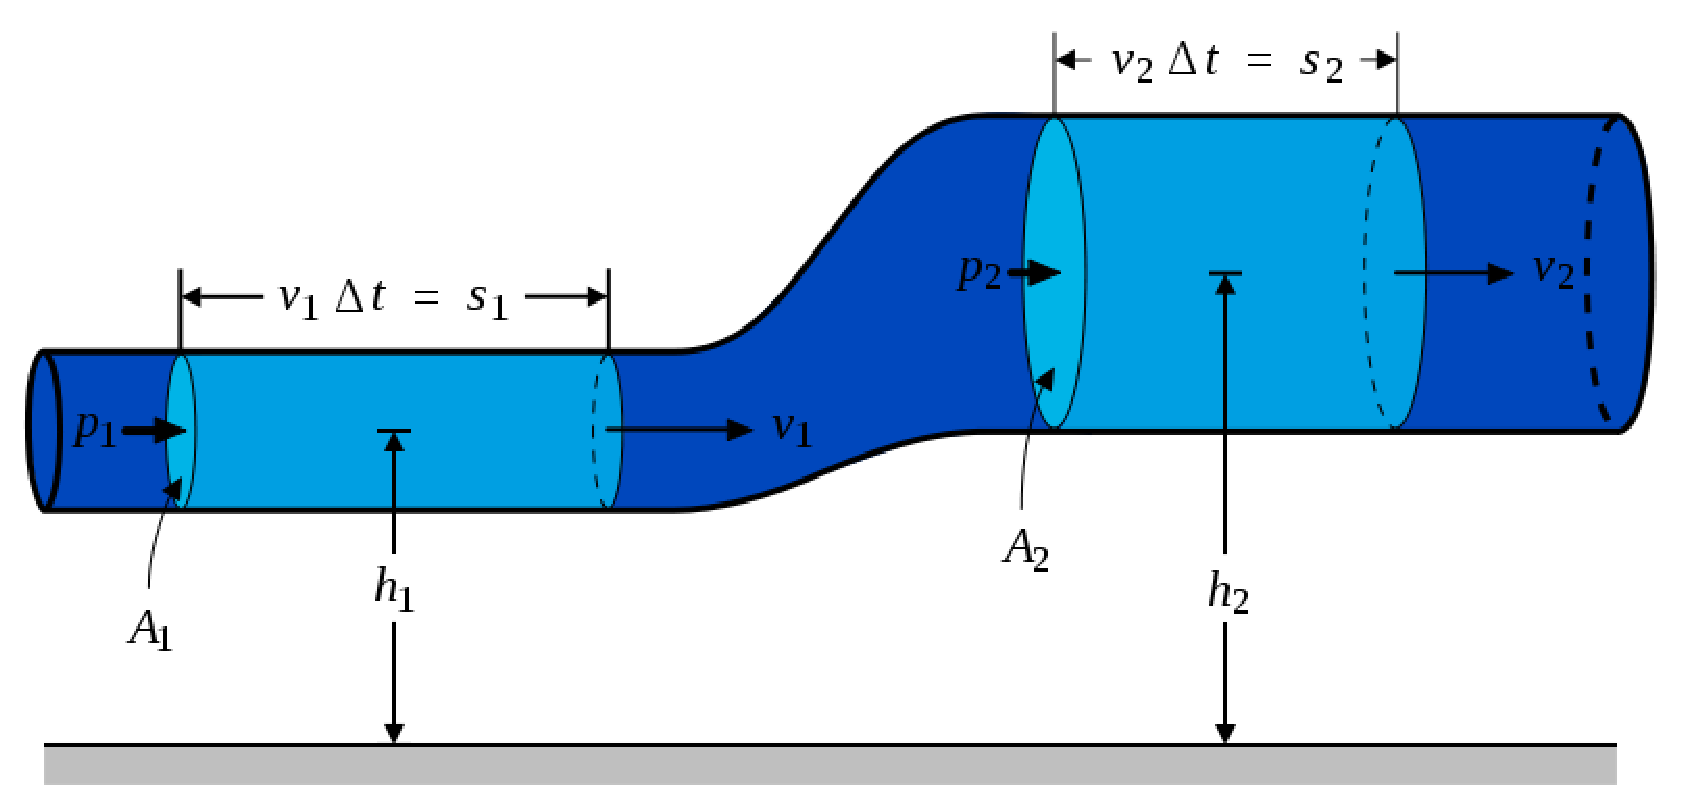
\includegraphics[scale=0.35]
		{figs/790px-BernoullisLawDerivationDiagram.eps}

	\caption{Sample image from Wikipedia}	% CAPTION FOR THE FIGURE
	\label{fig:wiki01}						% LABEL THE FIGURE FOR REFERENCING
\end{figure}								% END THE FIGURE

And sample subfigures:
\begin{figure}[!ht]	% FORCE LOCATION TO HERE (h), OR TOP OF PAGE (t)
	\centering								% CENTER THE FIGURE

	% LINK TO THE ACTUAL IMAGES.  EACH SUB-FIGURE HAS ITS OWN CAPTION 
	% DEFINED WITHIN THE [] FOLLOWING \subfloat
	\subfigure[From Wikipedia]{\label{fig:1a}
			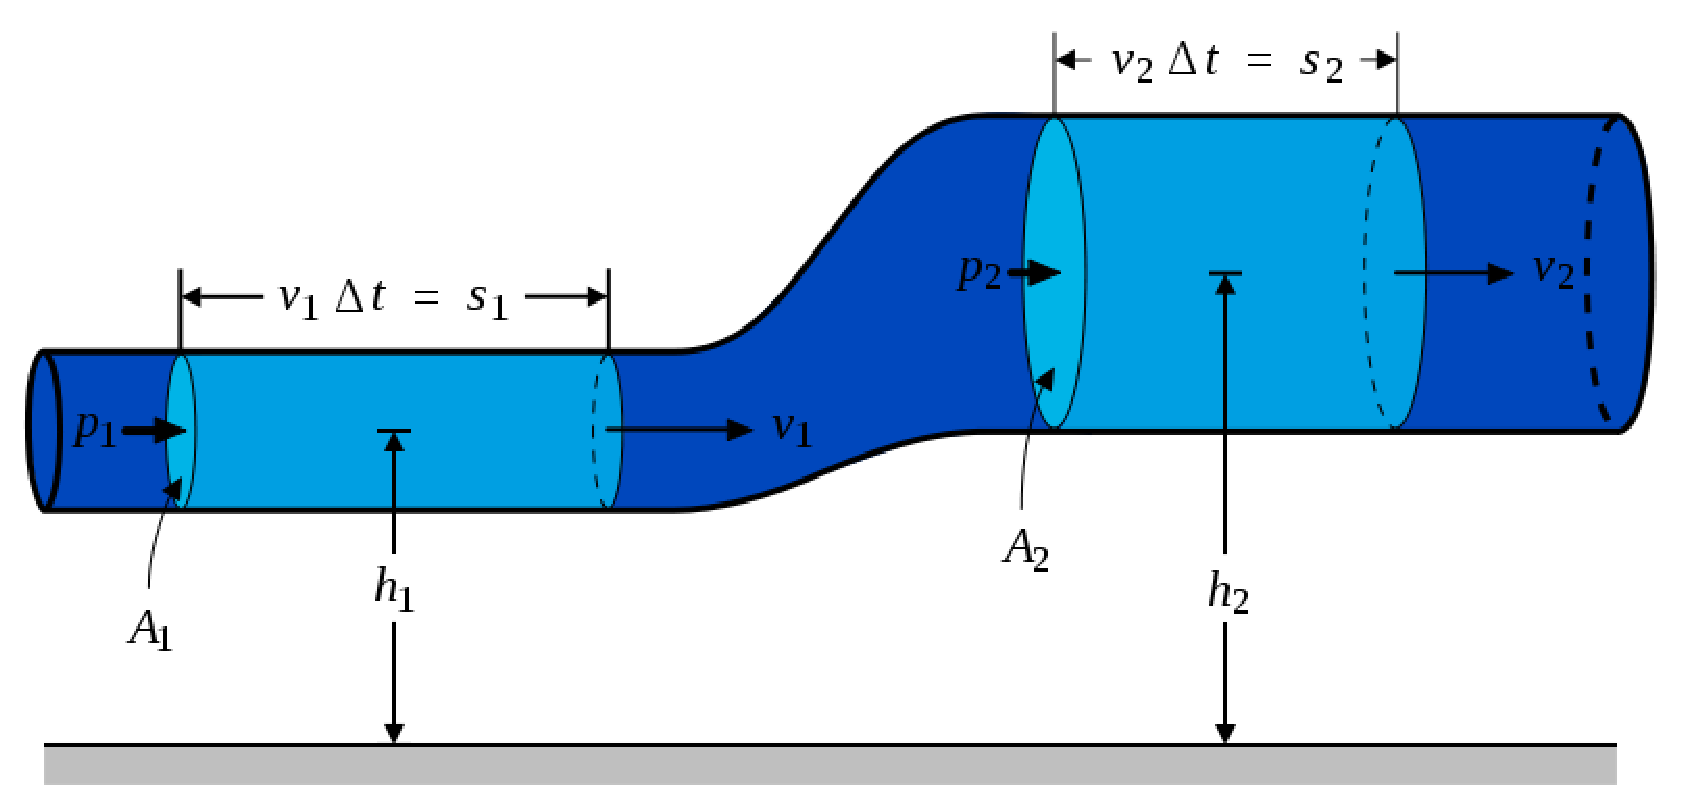
\includegraphics[width=0.3\textwidth]
			{figs/790px-BernoullisLawDerivationDiagram.eps}}
	\subfigure[Also from Wikipedia]{\label{fig:1b}
			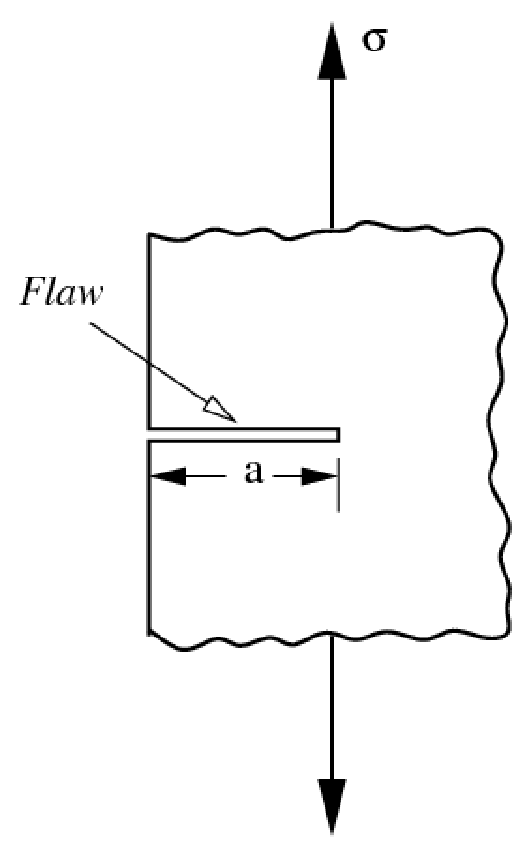
\includegraphics[width=0.3\textwidth]{figs/EdgeCrack2D.eps}}

	\caption{Subfigure Example}			% CAPTION FOR THE ENTIRE SET OF FIGURES
	\label{fig:sub01}					% LABEL THE ENTIRE FIGURE SET FOR 
										% REFERENCING
\end{figure}							% END THE FIGURE


\newpage
\section{Tables}

Here is an example of using a longtable environment.

\begin{center}
	\begin{longtable} {| c | c | c | c |}
	
	\caption{Hal compute nodes} \\
	
	\hline 
	\textbf{Node} & \textbf{Number of Cores} & \textbf{Processor Speed} & \textbf{Memory}\\
	  			  &							 & \textbf{[MHz]}			& \textbf{[GB]} \\
	\hline
	\endfirsthead
	
	\multicolumn{4}{c}%
	{{\bfseries \tablename\ \thetable{} -- continued from previous page}} \\
	\hline 
	\textbf{Node} & \textbf{Number of Cores} & \textbf{Processor Speed} & \textbf{Memory} \\
	  			  &							 & \textbf{[MHz]}			& \textbf{[GB]} \\
	\hline
	\endhead
	
	\hline \multicolumn{4}{|r|}{{Continued on next page}} \\ \hline
	\endfoot
	
	\hline
	\endlastfoot

		master & 4 & 2593 & 2.83 \\ \hline
		1	   & 1 & 2000 & 0.98 \\ \hline
		2	   & 1 & 2000 & 0.98 \\ \hline
		3	   & 1 & 2000 & 0.98 \\ \hline
		4	   & 1 & 2000 & 0.98 \\ \hline
		5	   & 1 & 2000 & 0.98 \\ \hline
		6	   & 1 & 2000 & 0.98 \\ \hline
		7	   & 1 & 2000 & 0.98 \\ \hline
		8	   & 1 & 2000 & 0.98 \\ \hline
		9	   & 1 & 2000 & 0.98 \\ \hline
		10	   & 1 & 2000 & 0.98 \\ \hline
		11	   & 1 & 2000 & 0.98 \\ \hline
		12	   & 1 & 2000 & 0.98 \\ \hline
		13	   & 1 & 2000 & 0.98 \\ \hline
		14	   & 1 & 2000 & 0.98 \\ \hline
		15	   & 1 & 2000 & 0.98 \\ \hline
		16	   & 1 & 2000 & 0.98 \\ \hline
		17	   & 1 & 2000 & 0.98 \\ \hline
		18	   & 1 & 2000 & 0.98 \\ \hline
		19	   & 1 & 2000 & 0.98 \\ \hline
		20	   & 1 & 2000 & 0.98 \\ \hline
		21	   & 1 & 2000 & 0.98 \\ \hline
		22	   & 1 & 2000 & 0.98 \\ \hline
		23	   & 1 & 2000 & 0.98 \\ \hline
		24	   & 1 & 2000 & 0.98 \\ \hline
		25	   & 1 & 2000 & 0.98 \\ \hline
		26	   & 1 & 2000 & 0.98 \\ \hline
		27	   & 1 & 2000 & 0.98 \\ \hline
		28	   & 1 & 2000 & 0.98 \\ \hline
		29	   & 1 & 2000 & 0.98 \\ \hline
		30	   & 1 & 2000 & 0.98 \\ \hline
		31	   & 1 & 2000 & 0.98 \\ \hline
		
	\end{longtable}
	\label{tbl:table01}
\end{center}


\newpage
\section{Sample listing}

Here is an example of the listing environment.  In listing \ref{lst:openmp} it
is displaying source code.  I can also directly-reference lines, such as line
\ref{lbl:lst_pragma}, where the OpenMP pragma statement resides.  Notice how the
label text doesn't appear in the listing, due to the ``escapeinside'' option set
in main.tex.

\begin{lstlisting}[caption=Implementation of OpenMP in the reconstructioncode code,label=lst:openmp]
if(GetNThreads() > 1){
	// LOOP THROUGH EACH RECONSTRUCTED PLANE (PARALLEL EXECUTION)
	omp_set_num_threads(GetNThreads());

	#pragma omp parallel for private(ztomo) (*@\label{lbl:lst_pragma}@*)
	for(int n=0; n<volume.GetRes(3); n++){
		if(nplanes == 1){
			ztomo = zmin;
		}
		if(volume.GetRes(3) > 1){
			ztomo = zmin + (zmax - zmin)/((T)nplanes - 1.0)*(T)n;
		}

		// CALL FUNCTION TO BUILD PLANE
		ParallelFCN_ISOCentricFilter(n,ztomo);

		#pragma omp atomic
		planescompleted++;
	}

} else {
	// LOOP THROUGH EACH RECONSTRUCTED PLANE (SERIAL EXECUTION)
	for(int n=0; n<volume.GetRes(3); n++){
		if(volume.GetRes(3) == 1){
			ztomo = zmin;
		}
		if(volume.GetRes(3) > 1){
			ztomo = zmin + (zmax - zmin)/((T)nplanes - 1.0)*(T)n;
		}

		// CALL FUNCTION TO BUILD PLANE
		ParallelFCN_ISOCentricFilter(n,ztomo);

		planescompleted++;
	}
}
\end{lstlisting}



% =============================================================================
% ========
% ========			APPENDICES
% ========
% =============================================================================
% COMMENT-OUT UNNECESSARY APPENDICES AS NEEDED.  NOTE THAT THE \appendix
% COMMAND IS LOCATED HERE, SO EACH APPENDIX FILE CAN BEGIN WITH A \chapter OR
% \section COMMAND.  THIS ALLOWS FOR EASIER INCLUSION/EXCLUSION/REARRANGEMENT
% OF APPENDICES BY NOT REQUIRING THE FIRST-LISTED INCLUDE FILE TO HAVE THE 
% \appendix COMMAND.  ALSO NOTE THAT \appendix WILL FORCE THE APPENDICES TO
% BEGIN ON A NEW PAGE, SO A \newpage COMMAND IS NOT NEEDED.
\appendix
% NOTE THAT THERE IS NO \appendix COMMAND IN THIS APPENDIX FILE (OR ANY OTHERS,
% SHOULD YOU CREATE MORE).  THE \appendix COMMAND IS IN main.tex BEFORE
% INCLUDING THE APPENDIX FILES SUCH AS THIS ONE.


\section{Appendix: Title}
\label{appA}

Appendix A material here.



\section{Appendix: Title2}
\label{appB}

Appendix B material here. 

\begin{verbatim}
Code here
\end{verbatim}



% =============================================================================
% ========
% ========			BIBLIOGRAPHY
% ========
% =============================================================================
\raggedright
\bibliographystyle{plain}
\bibliography{sources}

% OTHER BIBLIOGRAPHY STYLE OPTIONS:
%	- aiaa		AMERICAN INSTITUTE OF AERONAUTICS AND ASTRONAUTICS
%	- ams		AMERICAN MATHEMATICS SOCIETY
%	- apacite	AMERICAN PSYCHOLOGICAL ASSOCIATION
%


% =============================================================================
% ========
% ========			INDEX
% ========
% =============================================================================
% COMMENT-OUT THESE LINES IF NO INDEX IS NEEDED
\newpage
\printindex

\end{document}

% =============================================================================
% ========
% ========			REFERENCE NOTES
% ========
% =============================================================================
%
% INCLUDED REFERENCES:
%	- NOMENCLATURE
%	- INDEX
%	- LISTS
%	- TABLES
%	- FIGURES/SUBFIGURES
%
% THE END OF THIS LONG COMMENT-BLOCK CONTAINS ``CLEAN'' VERSIONS OF TABLE AND
% FIGURE EXAMPLES TO ALLOW FOR EASIER COPYING AND PASTING WITHOUT UNNECESSARY
% COMMENTS.
%
%
%
%
%	======================== NOMENCLATURE / INDEX =========================
%
% NOMENCLATURE IN-DOCUMENT USEAGE:
% 	\nomenclature{symbol}{definition}
%
% SAMPLE NOMENCLATURE (NOTE THE USE OF $'S TO GENERATE GREEK LETTERS AND
% SYMBOLS IN MATH-MODE):
% 		\nomenclature{$\alpha$}{Angular Acceleration}
% 		\nomenclature{$\gamma_{st}$}{Specific weight of steel}
% 		\nomenclature{$\ddot{S}_1$}{Acceleration of bullet, Phase I}
%
% INDEX IN-DOCUMENT USAGE:
%	\index{item}						--- SINGLE-LEVEL REFERENCE
%	\index{item!subitem}				--- SUB-LEVEL REFERENCE
%	\index{item!subitem!subsubitem}		--- NOTE: ONLY THREE LEVELS ALLOWED
%	\index{item|(}						--- BEGIN SECTION-REFERENCE
%	\index{item|)}						--- END SECTION-REFERENCE
%	\index{item|see{item2}}				--- CROSS-REFERENCE (NO PAGE NUMBER GIVEN)
%	\index{itempos@itemtext}			--- USE SPECIFIC TEXT itempos FOR CORRECT
% 											PLACEMENT OF itemtext
%							 THIS IS USEFUL FOR GREEK LETTERS: \index{alpha@$\alpha$}
%							 SO THAT \alpha IS ORDERED LIKE alpha
%							 ALSO USEFUL FOR FORMATTING WITHIN INDEX 
%							 (SUCH AS USING \bf)
%	\index{item|ii}						--- ITALICIZE THIS PARTICULAR REFERENCE
%											(OTHER REFERENCES WILL BE NORMAL FONT),
%											SUCH AS FOR DENOTING THE PRIMARY 
%											REFERENCE)
%	\index{item|nn}						--- ADD n TO THE PAGE NUMBER TO DENOTE THE
%											REFERENCE TO A FOOTNOTE
%
%
% SAMPLE INDEX (PLACES AN ENTRY OF 'text' IN THE INDEX WHICH REFERENCES THIS
% OCCURRANCE OF 'My test in the paragraph goes here.'):
% 		My test in the paragraph goes here. \index{text}
%
% TO GENERATE NOMENCLATURE/INDEX, FIRST LATEX-BUILD AS NORMAL (THIS FINDS THE
% NOMENCLATURE AND INDEX ITEMS). THEN RUN 
%
% 		'LaTeX_nomenclature_index.sh [file_name] [1/2/3]'
%
% IN THE TERMINAL (THIS GENERATES THE LIST(S)), WHERE	[file_name] IS THE NAME 
% OF THE MAIN DOCUMENT FILE (NO *.TEX EXTENSION) AND 1/2/3 DENOTES WHAT SHOULD
% BE COMPILED:
%						1 --- NOMENCLATURE (NO INDEX)
%						2 --- INDEX (NO NOMENCLATURE)
%						3 --- BOTH NOMENCLATURE AND INDEX
% FINALLY, BUILD THE LATEX DOCUMENT AGAIN (THIS ACTUALLY PUTS THE LISTS INTO THE
% DOCUMENT)
% 
%
%
% 	========================= LISTS ======================================
%
% LISTS REFERENCE:
% BULLETED LISTS USE THE {itemize} ENVIRONMENT.
% NUMBERED LISTS USE THE {enumerate} ENVIRONMENT.
% IN BOTH CASES, A \item COMMAND DELINEATES EACH ITEM.  LINE-BREAKS/PARAGRAPH-BREAKS
% DO NOT INDUCE BULLET POINTS OR NUMBERS.  INDENTATION IN CODE DOES NOT AFFECT
% COMPILATION, BUT IS RECOMMENDED TO IMPROVE CODE READABILITY.
%
% BULLETED EXAMPLE:
%	\begin{itemize}
%		\item This is the first bullet.
%		\item This is the second bullet.
%	\end{itemize}
%
% NUMBERED EXAMPLE:
%	\begin{enumerate}
%		\item This item has ``1.'' by it.
%		\item This item has ``2.'' by it.
%	\end{enumerate}
%
% ENVIRONMENTS CAN BE NESTED TO CREATE MULTI-LEVEL LISTS.  BULLETED AND NUMBERED
% CAN BE MIXED, AND AN \end COMMAND MUST APPEAR TO MATCH EACH \begin COMMAND.
%
% NESTED EXAMPLE:
%	\begin{enumerate}
%		\item First item.  Line identified by a number.
%		\begin{itemize}
%			\item Bulleted item beneath the first item.
%			\item Another bulleted item beneath the first item.
%		\end{itemize}
%
%		\item Second numbered item.
%	\end{enumerate}
% 
% 
%
%
%	============================ TABLES ===================================
%
% TABLE-MAKING REFERENCE:
%	\begin{center}
%		% BEGIN LONGTABLE ENVIRONMENT WITH FOUR CENTERED COLUMNS
%		\begin{longtable} {| c | c | c | c |}
%		
%		% PROVIDE A CAPTION.  MUST INCLUDE THE ``\\" AFTER.
%		\caption{Hal Details} \\
%		
%		% DEFINE THE HEADER ON THE FIRST PAGE OF THE TABLE.  THIS IS BUILT JUST
%		% LIKE ANY OTHER PORTION OF THE TABLE.  LEADING/TRAILING ``\hline'' IS
%		% RECOMMENDED.  THIS EXAMPLE USES MULTIPLE ROWS FOR THE HEADER IN ORDER
%		% TO KEEP IT FROM GETTING TOO WIDE.
%		\hline 
%		\textbf{Node} & \textbf{Number of Cores} & \textbf{Processor Speed} & \textbf{Memory}\\
%		  			  &							 & \textbf{[MHz]}			& \textbf{[GB]} \\
%		\hline
%		\endfirsthead
%	
%		% DEFINE THE HEADER TO APPEAR ON SUBSEQUENT PAGES, AS NECESSARY.  LIKELY,
%		% THIS SHOULD MATCH THE FIRST HEADER.  NO DIFFERENCE IS MADE BETWEEN THE 
%		% SECOND-PAGE HEADER AND THIRD-PAGE HEADER (OR ANY OTER PAGE).  ONLY 
%		% DIFFERENCE THAT CAN BE MADE IS FIRST PAGE VS. ALL OTHER PAGES.
%		\multicolumn{4}{c}%
%		{{\bfseries \tablename\ \thetable{} -- continued from previous page}} \\
%		\hline 
%		\textbf{Node} & \textbf{Number of Cores} & \textbf{Processor Speed} & \textbf{Memory} \\
%		  			  &							 & \textbf{[MHz]}			& \textbf{[GB]} \\
%		\hline
%		\endhead
%	
%		% DEFINE THE FOOTER TO BE USED IN THE EVENT THAT THE TABLE SPANS MULTIPLE
%		% PAGES.
%		\hline \multicolumn{4}{|r|}{{Continued on next page}} \\ \hline
%		\endfoot
%	
%		% DEFINE FOOTER TO APPEAR AT THE END OF THE TABLE (REGARDLESS OF WHAT PAGE
%		% IT FALLS-ON).
%		\hline
%		\endlastfoot
%
%		% ENTER THE TABLE DATA, WITH COLUMNS SEPARATED BY ``&'', LIKE NORMAL.
%		% THE FORMAT HERE AUTOMATICALLY PLACES A LINE BETWEEN ROWS WITH THE
%		% ``\\ \hline'' COMBINATION.
%		master & 4 & 2593 & 2.83 \\ \hline
%		1	   & 1 & 2000 & 0.98 \\ \hline
%		
%		\end{longtable}
%		\label{tbl:haldetails}
%	\end{center}
%
%
%
%	============================ FIGURES / SUBFIGURES ====================
% FIGURE REFERENCE:
%	\begin{figure}[!ht]	% FORCE LOCATION TO HERE (h), OR TOP OF PAGE (t)
%		\centering								% CENTER THE FIGURE
%
%		% LINK TO THE ACTUAL IMAGE
%		\includegraphics[scale=0.35]{figures.dir/NSAFlowchart}
%
%		\caption{An Awesome Caption}		% CAPTION FOR THE FIGURE
%		\label{fig1}							% LABEL THE FIGURE FOR REFERENCING
%	\end{figure}								% END THE FIGURE
%
%
%
% SUBFIGURE REFERENCE:
%	\begin{figure}[!ht]	% FORCE LOCATION TO HERE (h), OR TOP OF PAGE (t)
%		\centering								% CENTER THE FIGURE
%
%		% LINK TO THE ACTUAL IMAGES.  EACH SUB-FIGURE HAS ITS OWN CAPTION 
%		% DEFINED WITHIN THE [] FOLLOWING \subfloat
%		\subfigure[Figure 1a]{\label{fig:1a}
%				\includegraphics[width=0.3\textwidth]{firstimage}}
%		\subfigure[Figure 1b]{\label{fig:1a}
%				\includegraphics[width=0.3\textwidth]{secondimage}}
%		\subfigure[Figure 1c]{\label{fig:1a}
%				\includegraphics[width=0.3\textwidth]{thirdimage}}
%
%		\caption{An Awesome Caption}		% CAPTION FOR THE ENTIRE SET OF FIGURES
%		\label{fig1}						% LABEL THE ENTIRE FIGURE SET FOR 
%											% REFERENCING
%	\end{figure}							% END THE FIGURE
%
%
%
%
%
% =============================================================================
% ========
% ========			``CLEAN'' ITEMS FOR EASIER COPY/PASTE
% ========
% =============================================================================
%
% TABLE: NO HEADER ROW
%\begin{center}
%	\begin{longtable} {| c | c |}
%	\caption{Hal Details} \\
%	
%	\hline 
%	\endfirsthead
%	
%	\multicolumn{2}{c}%
%	{{\bfseries \tablename\ \thetable{} -- continued from previous page}} \\
%	\hline 
%	\endhead
%	
%	\hline \multicolumn{2}{|r|}{{Continued on next page}} \\ \hline
%	\endfoot
%	
%	\hline
%	\endlastfoot
%	
%	Operating System	& Red Hat Enterprise Linux 64-bit \\ \hline
%	CPU					& 1x AMD Quad-Core @ 2.6 GHz \\ \hline
%	System Memory		& 3 GB \\ \hline
%	System Storage		& 3.5 TB \\ \hline
%	RAM Disk			& 24 GB \\ \hline
%	MPI Implementation	& MPICH \\ \hline
%	
%	\end{longtable}
%	\label{tbl:table01}
%\end{center}
%
%
% TABLE: WITH HEADER ROW(S)
%\begin{center}
%	\begin{longtable} {| c | c | c | c |}
%	
%	\caption{Hal compute nodes} \\
%	
%	\hline 
%	\textbf{Node} & \textbf{Number of Cores} & \textbf{Processor Speed} & \textbf{Memory}\\
%	  			  &							 & \textbf{[MHz]}			& \textbf{[GB]} \\
%	\hline
%	\endfirsthead
%	
%	\multicolumn{4}{c}%
%	{{\bfseries \tablename\ \thetable{} -- continued from previous page}} \\
%	\hline 
%	\textbf{Node} & \textbf{Number of Cores} & \textbf{Processor Speed} & \textbf{Memory} \\
%	  			  &							 & \textbf{[MHz]}			& \textbf{[GB]} \\
%	\hline
%	\endhead
%	
%	\hline \multicolumn{4}{|r|}{{Continued on next page}} \\ \hline
%	\endfoot
%	
%	\hline
%	\endlastfoot
%
%		master & 4 & 2593 & 2.83 \\ \hline
%		1	   & 1 & 2000 & 0.98 \\ \hline
%		
%	\end{longtable}
%	\label{tbl:table01}
%\end{center}
%
%
% FIGURE / SUBFIGURE
%\begin{figure}[!ht]
%	\centering
%	% LINK TO THE ACTUAL IMAGE
%	\includegraphics[scale=0.35]{figures.dir/NSAFlowchart}
%	\caption{An Awesome Caption}
%	\label{fig1}
%\end{figure}
%
%
%
% SUBFIGURE REFERENCE:
%\begin{figure}[!ht]
%	\centering
%	\subfigure[Figure 1a]{\label{fig:1a}
%			\includegraphics[width=0.3\textwidth]{firstimage}}
%	\subfigure[Figure 1b]{\label{fig:1a}
%			\includegraphics[width=0.3\textwidth]{secondimage}}
%	\subfigure[Figure 1c]{\label{fig:1a}
%			\includegraphics[width=0.3\textwidth]{thirdimage}}
%	\caption{An Awesome Caption}
%	\label{fig1}
%\end{figure}
%
%